% Copyright (c) 2016, 2017 The ALF project.
% This is a part of the ALF project documentation.
% The ALF project documentation by the ALF contributors is licensed
% under a Creative Commons Attribution-ShareAlike 4.0 International License.
% For the licensing details of the documentation see license.CCBYSA.

% !TEX root = doc.tex

%------------------------------------------------------------
\subsubsection{Langevin dynamics}
%------------------------------------------------------------

Neglecting the  systematic error origination from the finite imaginary time step, the general from of the action reads:
\begin{equation}
   Z  =   \sum_{C}   e^{-S_{0,I} \left( \left\{ s_{i,\tau} \right\}  \right) }     \left( \prod_{k=1}^{M_V} \prod_{\tau=1}^{L_{\mathrm{Trotter}}} \gamma_{k,\tau} \right)
    e^{ N_{\mathrm{col}}\sum\limits_{s=1}^{N_{\mathrm{fl}}} \sum\limits_{k=1}^{M_V} \sum\limits_{\tau = 1}^{L_{\mathrm{Trotter}}}\sqrt{-\Delta \tau U_k}  \alpha_{k,s} \eta_{k,\tau} }  e^{ - S^{F}(C) }   \equiv \sum_{C} e^{-S(C)}
\end{equation}
where the fermionic part is  given by
\begin{equation}
e^{ - S^{F}(C) }  =  \prod_{s=1}^{N_{\mathrm{fl}}}\left[\det\left(  \mathds{1} + 
     \prod_{\tau=1}^{L_{\mathrm{Trotter}}}   
    \prod_{k=1}^{M_V}   e^{  \sqrt{ -\Delta \tau  U_k} \eta_{k,\tau} {\bm V}^{(ks)} }   \prod_{k=1}^{M_I}   e^{  -\Delta \tau s_{k,\tau}  {\bm I}^{(ks)}}  
     \prod_{k=1}^{M_T}   e^{-\Delta \tau {\bm T}^{(ks)}} 
     \right) \right]^{N_{\mathrm{col}}} .
\end{equation} 
To formulate both the Langevin dynamics as well as the Hybrid Monte Carlo, we will need  to estimate the fermion forces: 
\begin{equation}
	\frac { \partial S^F(C)}{\partial s_{k,\tau} }.
\end{equation}
The routine  \texttt{Langevin\_update} in the module \texttt{Langevin\_update\_mod.F90}   computes  thees forces  for a  general model and passes  them into a user defined routine in the Hamiltonian file  \texttt{ Ham\_Langevin\_update}  where the Langevin update is carried out.    Clearly, in this context 
$ s_{k,\tau}$  is a real valued quantity. 

Langevin dynamics  corresponds to a  stochastic differential equation   for the fields  $\pmb{s} \equiv \left\{s_{k,\tau} \right\}$. They acquire a Langevin time $\tl$  and satisfy the stochastic differential equation
\begin{equation}
   \ve{s}(\tl +  \delta \tl)    =    \ve{s}(\tl)    - \frac{\partial S(C) }{\partial    \ve{s}(\tl) }    \delta \tl     +\sqrt{2 \delta \tl } \ve{\eta}.
\end{equation}
Here, $  \ve{\eta}  $   are  independent Gaussian  stochastic variables  satisfying:
\begin{equation}
        \langle  \eta_{k,\tau} \rangle_{\eta}  = 0   \text{  and  }    \langle  \eta_{k,\tau}  \eta_{k',\tau'} \rangle_{\eta}  = \delta_{k,k'} \delta_{\tau,\tau'}
\end{equation}
We refer the reader to  Ref.~\cite{Gardiner}   for a more in depth introduction to stochastic differential equations.
To see that the above  indeed produced the desired probability distribution in the long Langevin time limit, we can transform the Langevin equation  to the corresponding Fokker-Plank one.  Let
$P(\ve{s}, \tl) $ be the distribution of fields at Langevin time $\tl$. Then,
\begin{equation}
        P(\ve{s}, \tl  + \delta \tl )    = \int D\ve{s}'  P  (\ve{s}', \tl  )    \langle    \delta \left(  \ve{s} - \left[ \ve{s}'   - \frac{\partial S(\ve{s}' )}{\partial    \ve{s}' }   \delta \tl     +\sqrt{2 \delta \tl } \pmb{\eta}  \right]    \right) \rangle_{\eta}
\end{equation}
where $\delta$ corresponds to the $L_{trot} M_I $  dimensional Dirac $\delta$-function.   Taylor expanding  up to order $\delta \tl$  and averaging over the stochastic variable yields:
\begin{eqnarray}
P(\ve{s}, \tl  + \delta \tl ) & &     = \int D\ve{s'}  P  (\ve{s}', \tl  )   \times  \\  & &  \left(   \delta \left(  \ve{s}' - \ve{s}   \right)
- \frac{\partial S(\ve{s'}) }{\partial    \ve{s'} }   \frac{\partial  }{\partial    \ve{s'} } \delta \left(  \ve{s}' - \ve{s} \right)  \delta \tl   +
   \frac{\partial  }{\partial    \ve{s'} }   \frac{\partial  }{\partial    \ve{s}' }  \delta \left(  \ve{s}' - \ve{s}\right)    \delta \tl
\right)  \nonumber   \\
  &&   + {\cal O}  \left(  \delta \tl^2 \right) \nonumber.
\end{eqnarray}
Partial integration  and taking the limit of infinitesimal time steps   gives the Fokker-Plank equation
\begin{equation}
         \frac{\partial  }{\partial   \tl}  P( \ve{s}, \tl)  =  \frac{\partial  }{\partial    \ve{s} }  \left( P( \ve{s}, \tl)  \frac{\partial S(\ve{s}) }{\partial     \ve{s} }   +
          \frac{\partial P(\ve{s},\tl) }{\partial     \ve{s} }
         \right)
\end{equation}
The stationary,  $ \frac{\partial  }{\partial   \tl}  P( \ve{s}, \tl) =0$,  normalizable,  solution to the above equation corresponds to the desired probability distribution:
\begin{equation}
          P(\ve{s}) =  \frac{ e^{ - S(\ve{s}) } }   {   \int D \ve{s}  e^{ - S(\ve{s}) } }.
\end{equation}
As mentioned above, Langevin dynamics will work well  provided that  the forces show  no  singularities.     The great advantage of such an updating scheme is that there is no rejection and  that all  fields are updated at each step.  The following points that highlight potential issues with Langevin dynamics are in order.
\begin{itemize}
\item   Langevin dynamics will be carried out at a finite  Langevin time step and thereby we have introduced a further source of systematic error.
\item   The factor $\sqrt{2 \delta \tl} $   multiplying the stochastic variable makes the  noise dominant  on short time scales.  On these times scales  Langevin dynamics essentially  corresponds to a random walk. This has the advantage that one can circumvent potential barriers, but  may render the updating scheme less  efficient than the hybrid molecular  dynamics approach.
\end{itemize}
In the code, we have adopted a  variable time step strategy. This is important since   the determinant has zeros and the forces  are unbounded.    The user   provides an upper bound to the force, \texttt{Max\_Force},  and  if the maximal force in a configuration \texttt{Max\_Force\_Conf}, is large than \texttt{Max\_Force} the time step  is rescaled as 
\begin{equation}
     \tilde{\delta \tl}   =  \frac{ \texttt{Max\_Force} *  \delta \tl }{\texttt{Max\_Force\_Conf}}.
\end{equation}
With the adaptive time  step,  averages are computed as: 
\begin{equation}
   \langle \hat{O} \rangle = \frac{ \sum_n (\delta \tl )_n \langle \langle \hat{O} \rangle   \rangle_{(C_n)}} {\sum_n (\delta \tl )_n } 
\end{equation}


We have tested the code for a 6-site Hubbard chain at half-filling  at $U/t = 4$,  $\beta t = 4$    and with periodic boundary conditions.   One can show that for this choice of boundary conditions the   forces are not bounded 
and to make sure that the program does not   crash we have  set \texttt{Max\_Force = 1.5}  


 The discrete  variable code gives
\begin{equation}
 \langle  \hat{H} \rangle  =  -3.468429   \pm     0.000726.
\end{equation} 
The Langevin code at $ \delta \tl = 0.001$  yields 
\begin{equation}
 \langle  \hat{H} \rangle  =  -3.456968   \pm   0.009886 
\end{equation} 
and at $ \delta \tl = 0.01$ 
\begin{equation}
 \langle  \hat{H} \rangle  = -3.495365    \pm  0.007281 
\end{equation} 
 At $ \delta \tl = 0.001$   the maximal force that occurred during the run was 
$ 112$, whereas at $ \delta \tl = 0.01$ it grew to $524$.    In both cases the average force was given by $0.45$.   For larger values of  $ \delta \tl $ the maximal force grows and the fluctuations on the energy become  larger.  
( $ \langle  \hat{H} \rangle  =  -3.718439    \pm   0.206469 $  at $ \delta \tl = 0.02$. For this parameter set  the maximal force we encountered during the run was of $1658$.)

Controlling Langevin dynamics when the action has logarithmic divergences is a challenge, and it is not clear  that the results will be satisfying.  For our specific problem we can solve this issue by considering open boundary conditions. Following an argument put forward in \cite{Assaad07}, we can show, using world lines, that the determinant is always positive.   In this case the  action does not  have logarithmic divergences and the Langevin dynamics works beautifully well, see Fig.~\ref{Langevin.fig}. 

\begin{figure}[H]
        \begin{center}
                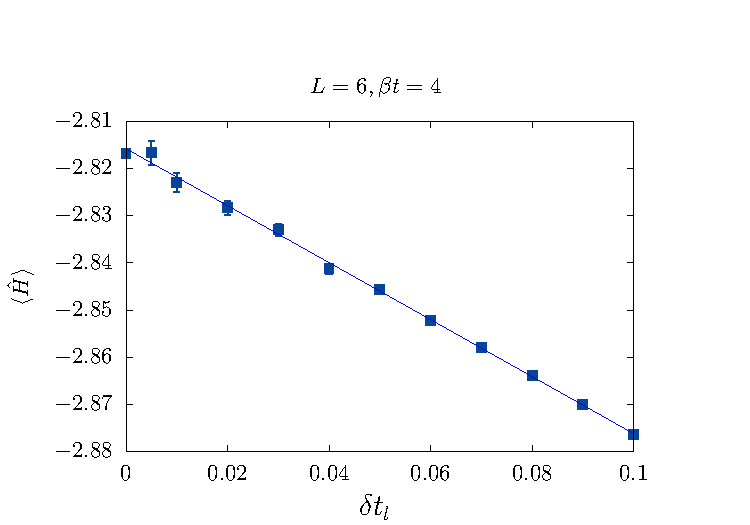
\includegraphics[scale=0.9]{Figures/Langevin.pdf}
            \end{center}
        \caption{\label{Langevin.fig}   Total energy for the 6-sites Hubbard chain at $U/t=4$, $\beta t = 4$ and with open boundary conditions.   Here one can show that the determinant is always positive such that  no   singularities occur in the action, and consequently the Langevin dynamics works very well.  The data point at $\delta \tl =0$ stems from running the  discrete  field code with coupling  of the field to the z-component of the magnetization.  The extrapolated value of the energy reads  $-2.87104   \pm 0.001144$ and the reference result from the discrete code is $  -2.871124   \pm  0.000389 $.  Throughout the runs the maximal force was always less than the threshold of 1.5.   }
\end{figure}


